%!TeX spelling=es_AR
\section{Transformaciones de fase en estado sólido}

Se trata de transformaciones en las que solo intervienen fase sólidas, a diferencia de la solidificación que es la transformación de la fase líquida.


Desde un punto de vista práctico estas intervienen en y están fuertemente relacionadas a los \textbf{tratamientos térmicos}.

Entender el diagrama de equilibrio es el primer paso para el entendimiento de la microestructura de una aleación metálica. Sin embargo, los diagramas de equilibrio no ofrecen información de tres aspectos importantes:

\begin{enumerate}
	\item Los {\bf tiempos} que necesitan las fases para comenzar y completarse
	\item Las {\bf morfologías} de las fases producto de la transformación. Morfología describe la distribución, tamaño y forma de las fases resultantes
	\item La posibilidad de la presencia de fases \textbf{fuera de equilibrio}
\end{enumerate}

Las transformaciones de fase se pueden clasificar en cinco principales

\begin{description}
	\item[Con difusión] Movimiento térmicamente activado (cada átomo se mueve de forma individual). Dos subtipos:
	\begin{description}
		\item[de largo alcance] Los átomos se mueven muchas distancias interatómicas. Las fases inicial y final \textbf{poseen distinta composición química} y pueden o no tener la misma red cristalina
		\item[de corto alcance]  Los átomos se mueven unas pocas distancias interatómicas. Fase inicial y final de igual composición química pero diferente estructura cristalina. Ejemplo: transformación alotrópica
	\end{description} 
	\item[Sin difusión] Movimiento cooperativo de un conjunto de átomos en forma coordinada y simultánea. Cada átomo ocupa un lugar bien determinado al final de la transformación
	\item[Mixtas] Generalmente en aleaciones pasa que un elemento experimenta difusión mientras que el otro puede moverse cooperativamente
\end{description}

\subsection{Transformación martensítica}

Se trata de una transformación militar/desplazativa. Los átomos se desplazan pequeñas distancias sin romper enlace con el vecino. Se crea una fase de igual composición pero con estructura nueva. Requiere una gran fuerza impulsora para desplazar un gran número de átomos. Es sin difusión y sin activar térmicamente. 


\subsection{Formación de fase nueva}

\begin{description}
	\item[Nucleación homogénea] Se necesita una gran fuerza impulsora para que ocurra la nucleación de una fase nueva en el interior de un grano. Ej: globulización
	\item[Nucleación heterogénea] Se producen los núcleos donde la barrera es menor como el borde de grano, sobre una pared que contiene la fase inicial o sobre zonas de alta densidad de dislocaciones (donde la barrera de nucleación es menor). Ej: acero inoxidables
	\item[Crecimiento] es una transformación de fase. Una vez que aparecen núcleos pueden crecer mediante la difusión 
\end{description}


\subsection{Transformación de precipitación}

Se trata de una transformación de fase en la que aparece una nueva fase a partir de otra sin que esta última desaparezca. Genera partículas nuevas, lo cual suele aumentar dureza. Más usado para aumentar dureza en materiales no-ferrosos. Si es lento el enfriamiento (menos $\Delta G$) entonces el precipitado aparece en el borde de grano.

\begin{itemize}
	\item Para lograr máxima dureza luego de envejecimiento el aleante no debe precipitar en los bordes de grano.
	\item Cuanto mayor sea la cantidad de aleante, mayor será la velocidad que se debe enfriar para evitar precipitación durante temple
	\item Cuanto más aleante, más duro
\end{itemize}

\subsubsection{Envejecimiento por precipitación}
Al comienzo de la precipitación se pierde dureza porque se consume la solución sólida para generar el precipitado. A medida que sigue la precipitación este comienza a dominar y se obtiene un endurecimiento notable por precipitación. 

Si se deja pasar suficiente tiempo ocurre el \textbf{sobre-envejecimiento} (zona III de la figura \ref{fig:orowan}). A partir de cierto tamaño de precipitado las dislocaciones tienden a rodear el precipitado en vez de cortarlo debido al a. Cuando sucede esto se generan lazos de dislocaciones alrededor de las partículas precipitadas. A partir de este punto el endurecimiento pasa a ser inversamente proporcional a la distancia promedio entre partículas. Esto es conocido como el \textbf{mecanismo de Orowan}.
  Las partículas se vuelven más gruesas (aumenta $r$) y hay más distancia entre ellas (aumenta $d$) así perdiendo la dureza.
 

\begin{figure}[htb]
	\centering
	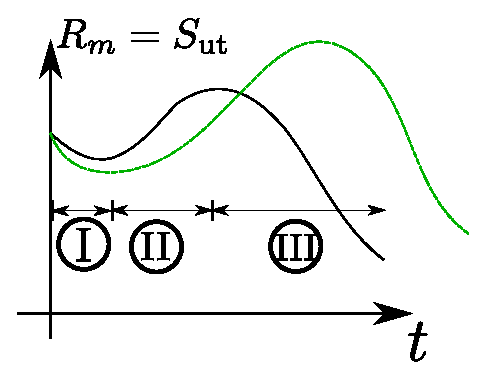
\includegraphics[width=0.5\linewidth]{fig/orowan.eps}
	\caption{Mecanismo de envejecimiento por precipitación. Las etapas corresponden a la curva negra sólida. La curva verde punteada representa un envejecimiento a una temperatura menor.}
	\label{fig:orowan}
\end{figure}

Las etapas de la figura \ref{fig:orowan} son enumeradas abajo. Se indica la relación de tensión a avance de dislocaciones con $\Delta \sigma$ donde $f$ es la fracción en volumen de partículas, $r$ el tamaño promedio de partícula y $d$ es la distancia promedio entre partículas. $\Delta \sigma$ es proporcional al aumento de dureza del material.

\begin{description}
	\item[I] Al comienzo del proceso el soluto difunde así permitiendo la precipitación. La difundición significa que se pierde la dureza aportada por solución sólida. $\Delta \sigma = \frac{f}{d}$
	\item[II]  Durante esta etapa el precipitado empieza a aportar dureza. El precipitado es fino y por ende las dislocaciones cortan las partículas. El endurecimiento es proporcional a la fracción en volumen y al tamaño promedio de las partículas. $\Delta \sigma = f \cdot r$
	\item[III] El precipitado se convierte suficientemente grueso al transcurrir tiempo como para que comienze a dominar el mecanismo de Orowan. $\Delta \sigma = \frac{1}{r\cdot d}$
\end{description}




